\chapter{ПОСТАНОВКА ЗАДАЧИ ПОЛУЧЕНИЯ, АНАЛИЗА И ОБРАБОТКИ ЭКСПЕРТНОЙ ИНФОРМАЦИИ} \label{chapt1}

\section{Возникновение области} \label{sect1_1}
В настоящее время в области IT набрало большую популярность системы удаленной поддержки информационной инфраструктуры, так называемый «Аутсорсинг». Ввиду развития рынка компаниям становится невыгодно держать свой штат службы поддержки, и они отдают свою инфраструктуру сторонней компании.
Большинство проблем, которые решает удаленная служба поддержки носят весьма тривиальный характер :
\begin{itemize}
	\item Установить приложение
	\item Переустановить приложение
	\item Решить проблему с доступом к тому или иному ресурсу
\end{itemize}
Данные проблемы решают специалисты технической поддержки. Обычно техническая поддержка делится на несколько линий:
\begin{enumerate}
	\item Первая линия. Решение уже известных, задокументированных проблем, работа напрямую с пользователем
	\item Вторая линия. Решение ранее неизвестных проблем
	\item Третья линия. Решение сложных и нетривиальных проблем
	\item Четвертая линия. Решение архитектурных проблем инфраструктуры
\end{enumerate}

Каждая линия поддержки представлена специалистами. В среднем команда, обслуживающая одного заказчика насчитывает 60 человек. Процентное соотношение специалистов разных линий поддержки отображено на Диаграмме \ref{img:ITSMTeamComposition}

\begin{figure} [h] 
  \center
  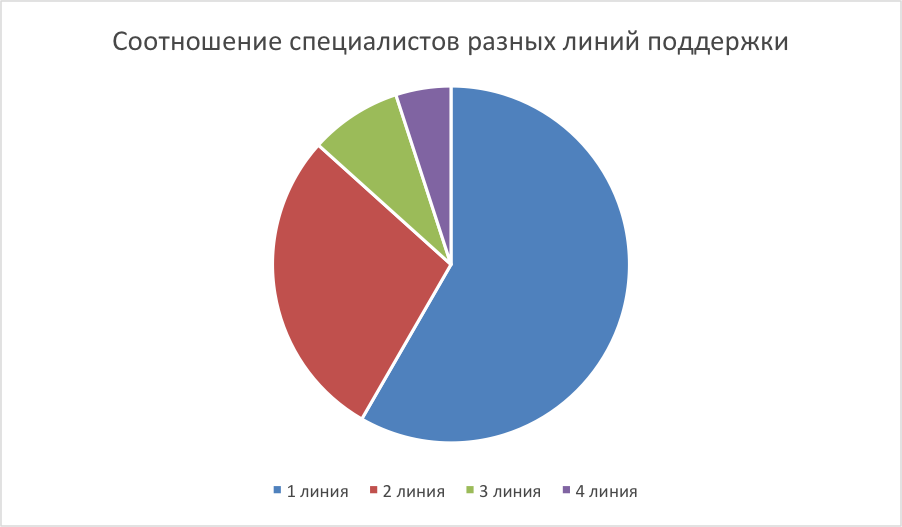
\includegraphics [scale=0.7] {ITSMTeamComposition}
  \caption{Диаграмма состава команд} 
  \label{img:ITSMTeamComposition}  
\end{figure}

Работа специалиста 1 линии поддержки состоит из множества рутинных и простых задач. На Диаграмме \ref{img:EngineerTasks}  показано соотношение разных типов проблем, встречающихся во время работы поддержки

\begin{figure} [h] 
  \center
  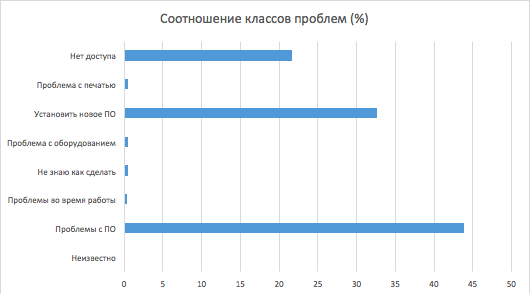
\includegraphics [scale=0.7] {EngineerTasks}
  \caption{Диаграмма соотношений типов проблем} 
  \label{img:EngineerTasks}  
\end{figure}

%\newpage
%============================================================================================================================

\section{Ссылки} \label{sect1_2}
Сошлёмся на библиографию. Одна ссылка: \cite{Sychev}. Две ссылки: \cite{Sokolov,Gaidaenko}. Много ссылок: \cite{Lermontov,Management,Borozda,Marketing,Constitution,FamilyCode,Gost.7.0.53,Razumovski,Lagkueva,Pokrovski,Sirotko,Lukina,Methodology,Encyclopedia,Nasirova,Berestova,Kriger}. И ещё немного ссылок: \cite{Article,Book,Booklet,Conference,Inbook,Incollection,Manual,Mastersthesis,Misc,Phdthesis,Proceedings,Techreport,Unpublished}.

Сошлёмся на приложения: Приложение \ref{AppendixA}, Приложение \ref{AppendixB2}.

Сошлёмся на формулу: формула \eqref{eq:equation1}.

Сошлёмся на изображение: рисунок \ref{img:knuth}.

%\newpage
%============================================================================================================================

\section{Формулы} \label{sect1_3}

Благодаря пакету \textit{icomma}, \LaTeX~одинаково хорошо воспринимает в качестве десятичного разделителя и запятую ($3,1415$), и точку ($3.1415$).

\subsection{Ненумерованные одиночные формулы} \label{subsect1_3_1}

Вот так может выглядеть формула, которую необходимо вставить в строку по тексту: $x \approx \sin x$ при $x \to 0$.

А вот так выглядит ненумерованая отдельностоящая формула c подстрочными и надстрочными индексами:
$$
(x_1+x_2)^2 = x_1^2 + 2 x_1 x_2 + x_2^2
$$

При использовании дробей формулы могут получаться очень высокие:
$$
  \frac{1}{\sqrt(2)+
  \displaystyle\frac{1}{\sqrt{2}+
  \displaystyle\frac{1}{\sqrt{2}+\cdots}}}
$$

В формулах можно использовать греческие буквы:
$$
\alpha\beta\gamma\delta\epsilon\varepsilon\zeta\eta\theta\vartheta\iota\kappa\lambda\\mu\nu\xi\pi\varpi\rho\varrho\sigma\varsigma\tau\upsilon\phi\varphi\chi\psi\omega\Gamma\Delta\Theta\Lambda\Xi\Pi\Sigma\Upsilon\Phi\Psi\Omega
$$

%\newpage
%============================================================================================================================

\subsection{Ненумерованные многострочные формулы} \label{subsect1_3_2}

Вот так можно написать две формулы, не нумеруя их, чтобы знаки равно были строго друг под другом:
\begin{eqnarray}
  f_W & = & \min \left( 1, \max \left( 0, \frac{W_{soil} / W_{max}}{W_{crit}} \right)  \right), \nonumber \\
  f_T & = & \min \left( 1, \max \left( 0, \frac{T_s / T_{melt}}{T_{crit}} \right)  \right), \nonumber
\end{eqnarray}

Можно использовать разные математические алфавиты:
\begin{eqnarray}
\mathcal{ABCDEFGHIJKLMNOPQRSTUVWXYZ} \nonumber \\
\mathfrak{ABCDEFGHIJKLMNOPQRSTUVWXYZ} \nonumber \\
\mathbb{ABCDEFGHIJKLMNOPQRSTUVWXYZ} \nonumber
\end{eqnarray}

Посмотрим на систему уравнений на примере аттрактора Лоренца:

$$
\left\{
  \begin{array}{rl}
    \dot x = & \sigma (y-x) \\
    \dot y = & x (r - z) - y \\
    \dot z = & xy - bz
  \end{array}
\right.
$$

А для вёрстки матриц удобно использовать многоточия:
$$
\left(
  \begin{array}{ccc}
  	a_{11} & \ldots & a_{1n} \\
  	\vdots & \ddots & \vdots \\
  	a_{n1} & \ldots & a_{nn} \\
  \end{array}
\right)
$$


%\newpage
%============================================================================================================================
\subsection{Нумерованные формулы} \label{subsect1_3_3}

А вот так пишется нумерованая формула:
\begin{equation}
  \label{eq:equation1}
  e = \lim_{n \to \infty} \left( 1+\frac{1}{n} \right) ^n
\end{equation}

Нумерованых формул может быть несколько:
\begin{equation}
  \label{eq:equation2}
  \lim_{n \to \infty} \sum_{k=1}^n \frac{1}{k^2} = \frac{\pi^2}{6}
\end{equation}

В последствии на формулы (\ref{eq:equation1}) и (\ref{eq:equation2}) можно ссылаться.

%\newpage
%============================================================================================================================

\clearpage
